% Options for packages loaded elsewhere
\PassOptionsToPackage{unicode}{hyperref}
\PassOptionsToPackage{hyphens}{url}
%
\documentclass[
]{article}
\usepackage{amsmath,amssymb}
\usepackage{iftex}
\ifPDFTeX
  \usepackage[T1]{fontenc}
  \usepackage[utf8]{inputenc}
  \usepackage{textcomp} % provide euro and other symbols
\else % if luatex or xetex
  \usepackage{unicode-math} % this also loads fontspec
  \defaultfontfeatures{Scale=MatchLowercase}
  \defaultfontfeatures[\rmfamily]{Ligatures=TeX,Scale=1}
\fi
\usepackage{lmodern}
\ifPDFTeX\else
  % xetex/luatex font selection
\fi
% Use upquote if available, for straight quotes in verbatim environments
\IfFileExists{upquote.sty}{\usepackage{upquote}}{}
\IfFileExists{microtype.sty}{% use microtype if available
  \usepackage[]{microtype}
  \UseMicrotypeSet[protrusion]{basicmath} % disable protrusion for tt fonts
}{}
\makeatletter
\@ifundefined{KOMAClassName}{% if non-KOMA class
  \IfFileExists{parskip.sty}{%
    \usepackage{parskip}
  }{% else
    \setlength{\parindent}{0pt}
    \setlength{\parskip}{6pt plus 2pt minus 1pt}}
}{% if KOMA class
  \KOMAoptions{parskip=half}}
\makeatother
\usepackage{xcolor}
\usepackage[margin=1in]{geometry}
\usepackage{color}
\usepackage{fancyvrb}
\newcommand{\VerbBar}{|}
\newcommand{\VERB}{\Verb[commandchars=\\\{\}]}
\DefineVerbatimEnvironment{Highlighting}{Verbatim}{commandchars=\\\{\}}
% Add ',fontsize=\small' for more characters per line
\usepackage{framed}
\definecolor{shadecolor}{RGB}{248,248,248}
\newenvironment{Shaded}{\begin{snugshade}}{\end{snugshade}}
\newcommand{\AlertTok}[1]{\textcolor[rgb]{0.94,0.16,0.16}{#1}}
\newcommand{\AnnotationTok}[1]{\textcolor[rgb]{0.56,0.35,0.01}{\textbf{\textit{#1}}}}
\newcommand{\AttributeTok}[1]{\textcolor[rgb]{0.13,0.29,0.53}{#1}}
\newcommand{\BaseNTok}[1]{\textcolor[rgb]{0.00,0.00,0.81}{#1}}
\newcommand{\BuiltInTok}[1]{#1}
\newcommand{\CharTok}[1]{\textcolor[rgb]{0.31,0.60,0.02}{#1}}
\newcommand{\CommentTok}[1]{\textcolor[rgb]{0.56,0.35,0.01}{\textit{#1}}}
\newcommand{\CommentVarTok}[1]{\textcolor[rgb]{0.56,0.35,0.01}{\textbf{\textit{#1}}}}
\newcommand{\ConstantTok}[1]{\textcolor[rgb]{0.56,0.35,0.01}{#1}}
\newcommand{\ControlFlowTok}[1]{\textcolor[rgb]{0.13,0.29,0.53}{\textbf{#1}}}
\newcommand{\DataTypeTok}[1]{\textcolor[rgb]{0.13,0.29,0.53}{#1}}
\newcommand{\DecValTok}[1]{\textcolor[rgb]{0.00,0.00,0.81}{#1}}
\newcommand{\DocumentationTok}[1]{\textcolor[rgb]{0.56,0.35,0.01}{\textbf{\textit{#1}}}}
\newcommand{\ErrorTok}[1]{\textcolor[rgb]{0.64,0.00,0.00}{\textbf{#1}}}
\newcommand{\ExtensionTok}[1]{#1}
\newcommand{\FloatTok}[1]{\textcolor[rgb]{0.00,0.00,0.81}{#1}}
\newcommand{\FunctionTok}[1]{\textcolor[rgb]{0.13,0.29,0.53}{\textbf{#1}}}
\newcommand{\ImportTok}[1]{#1}
\newcommand{\InformationTok}[1]{\textcolor[rgb]{0.56,0.35,0.01}{\textbf{\textit{#1}}}}
\newcommand{\KeywordTok}[1]{\textcolor[rgb]{0.13,0.29,0.53}{\textbf{#1}}}
\newcommand{\NormalTok}[1]{#1}
\newcommand{\OperatorTok}[1]{\textcolor[rgb]{0.81,0.36,0.00}{\textbf{#1}}}
\newcommand{\OtherTok}[1]{\textcolor[rgb]{0.56,0.35,0.01}{#1}}
\newcommand{\PreprocessorTok}[1]{\textcolor[rgb]{0.56,0.35,0.01}{\textit{#1}}}
\newcommand{\RegionMarkerTok}[1]{#1}
\newcommand{\SpecialCharTok}[1]{\textcolor[rgb]{0.81,0.36,0.00}{\textbf{#1}}}
\newcommand{\SpecialStringTok}[1]{\textcolor[rgb]{0.31,0.60,0.02}{#1}}
\newcommand{\StringTok}[1]{\textcolor[rgb]{0.31,0.60,0.02}{#1}}
\newcommand{\VariableTok}[1]{\textcolor[rgb]{0.00,0.00,0.00}{#1}}
\newcommand{\VerbatimStringTok}[1]{\textcolor[rgb]{0.31,0.60,0.02}{#1}}
\newcommand{\WarningTok}[1]{\textcolor[rgb]{0.56,0.35,0.01}{\textbf{\textit{#1}}}}
\usepackage{graphicx}
\makeatletter
\def\maxwidth{\ifdim\Gin@nat@width>\linewidth\linewidth\else\Gin@nat@width\fi}
\def\maxheight{\ifdim\Gin@nat@height>\textheight\textheight\else\Gin@nat@height\fi}
\makeatother
% Scale images if necessary, so that they will not overflow the page
% margins by default, and it is still possible to overwrite the defaults
% using explicit options in \includegraphics[width, height, ...]{}
\setkeys{Gin}{width=\maxwidth,height=\maxheight,keepaspectratio}
% Set default figure placement to htbp
\makeatletter
\def\fps@figure{htbp}
\makeatother
\setlength{\emergencystretch}{3em} % prevent overfull lines
\providecommand{\tightlist}{%
  \setlength{\itemsep}{0pt}\setlength{\parskip}{0pt}}
\setcounter{secnumdepth}{-\maxdimen} % remove section numbering
\usepackage{titling}
\pretitle{\begin{center}\Large}
\posttitle{\end{center}\vspace{-0.5cm}}
\preauthor{\begin{center}\normalsize}
\postauthor{\end{center}\vspace{-0.5cm}}
\predate{\begin{center}\normalsize}
\postdate{\end{center}\vspace{-0.5cm}}
\ifLuaTeX
  \usepackage{selnolig}  % disable illegal ligatures
\fi
\IfFileExists{bookmark.sty}{\usepackage{bookmark}}{\usepackage{hyperref}}
\IfFileExists{xurl.sty}{\usepackage{xurl}}{} % add URL line breaks if available
\urlstyle{same}
\hypersetup{
  pdftitle={Laplace Transform for Network Analysis - Detailed Report},
  hidelinks,
  pdfcreator={LaTeX via pandoc}}

\title{Laplace Transform for Network Analysis - Detailed Report}
\author{}
\date{\vspace{-2.5em}}

\begin{document}
\maketitle

\hypertarget{section}{%
\section{}\label{section}}

Name: Karthik Dani \textbar{} USN: 1BM22MD022 \textbar{} Course: Network
Analysis \textbar{} Faculty: Dr.~Niranjan K R

\hypertarget{introduction}{%
\subsection{Introduction}\label{introduction}}

This report will carry out computationally finding the Laplace transform
of a signal, this task is performed in R with appropriate programming on
plotting the curves using \texttt{ggplot2}, manually calculating the
Laplace transform for visualisation purposes.

\hypertarget{theory}{%
\subsection{Theory}\label{theory}}

The Laplace transform is a powerful mathematical tool extensively used
in network analysis to analyze and solve linear time-invariant (LTI)
systems. In network analysis, it offers a way to simplify differential
equations describing circuit behavior into algebraic equations,
facilitating their analysis.

\begin{itemize}
\tightlist
\item
  \textbf{Definition}: The Laplace transform of a function \(f(t)\) is
  defined as the integral of the function multiplied by \(e^{-st}\),
  where \(s\) is a complex variable:
\end{itemize}

\[
F(s) = \int_0^{\infty} e^{-st} f(t) dt
\]

\begin{itemize}
\item
  \textbf{Impulse Response}: The Laplace transform provides a way to
  compute the impulse response of linear systems, which is crucial for
  understanding their dynamic behavior.
\item
  \textbf{Circuit Analysis}: In network analysis, Laplace transforms are
  extensively used to analyze electrical circuits. They help in
  determining voltage and current responses, transient and steady-state
  behaviors, and frequency-dependent characteristics of circuits.
\item
  \textbf{Transform Pairs}: Several common transform pairs exist, which
  are widely used in network analysis, such as the step function,
  impulse function, exponential function, and trigonometric functions.
\item
  \textbf{Applications}: Laplace transform finds applications in various
  fields, including control theory, signal processing, communication
  systems, and electrical engineering, making it a fundamental tool in
  network analysis and system theory.
\end{itemize}

\hypertarget{question}{%
\subsection{Question}\label{question}}

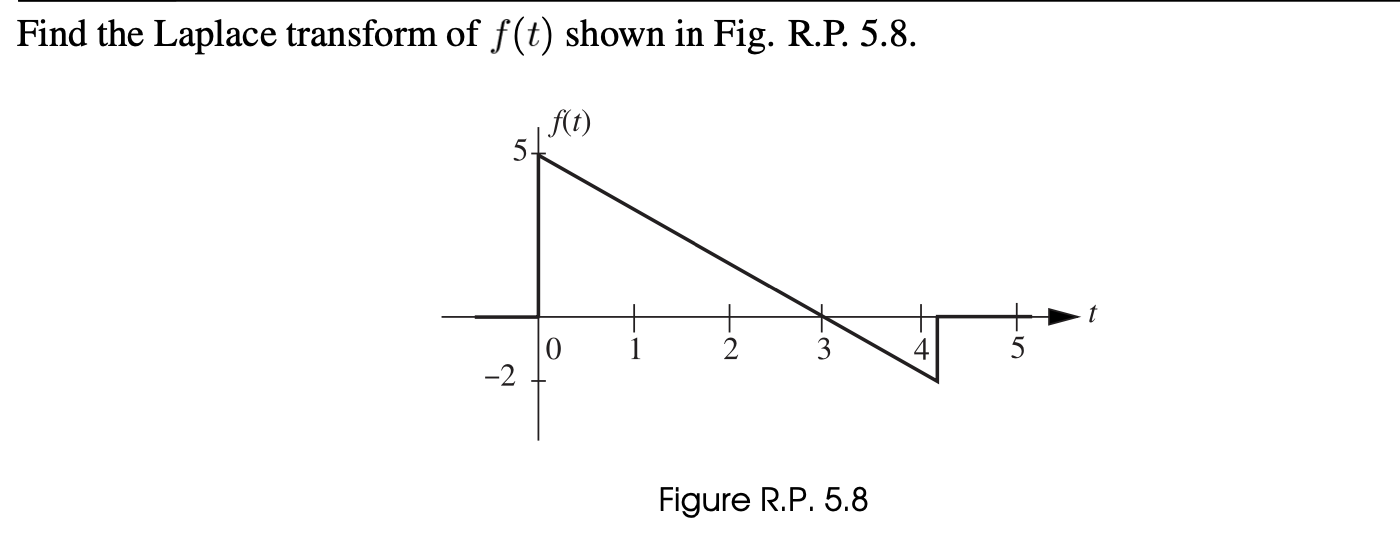
\includegraphics{question.png}

\hypertarget{solution}{%
\subsection{Solution}\label{solution}}

The equation of a straight line is \(y = mx + c\), where \(m\) = slope
of the line and \(c\) = intercept on y-axis.

Hence \(f(t) = \left(-\frac{5}{3}\right)t + 5\). When \(f(t) = -2\),
finding the value of \(t\) gives us,

\[-2 =(-\frac{5}{3})t + 5\]

Mathematically,

\[t = 4.2 \text{ seconds}\]

\hypertarget{load-packages}{%
\subsection{Load Packages}\label{load-packages}}

\begin{Shaded}
\begin{Highlighting}[]
\FunctionTok{library}\NormalTok{(ggplot2)}
\end{Highlighting}
\end{Shaded}

\hypertarget{define-the-function}{%
\subsection{Define the Function}\label{define-the-function}}

Let's define the function \(f(t)\) in R:

\begin{Shaded}
\begin{Highlighting}[]
\NormalTok{f }\OtherTok{\textless{}{-}} \ControlFlowTok{function}\NormalTok{(t) \{}
  \FunctionTok{return}\NormalTok{((}\SpecialCharTok{{-}}\DecValTok{5}\SpecialCharTok{/}\DecValTok{3}\NormalTok{)}\SpecialCharTok{*}\NormalTok{t }\SpecialCharTok{+} \DecValTok{5}\NormalTok{)}
\NormalTok{\}}
\end{Highlighting}
\end{Shaded}

\hypertarget{plot-the-function}{%
\subsection{Plot the Function}\label{plot-the-function}}

Now, let's plot \(f(t)\) over a suitable range. We'll use the range from
0 to 4.2 as given in the question:

\begin{Shaded}
\begin{Highlighting}[]
\NormalTok{t\_values }\OtherTok{\textless{}{-}} \FunctionTok{seq}\NormalTok{(}\DecValTok{0}\NormalTok{, }\FloatTok{4.2}\NormalTok{, }\AttributeTok{by =} \FloatTok{0.01}\NormalTok{)}
\NormalTok{f\_values }\OtherTok{\textless{}{-}} \FunctionTok{f}\NormalTok{(t\_values)}

\NormalTok{df }\OtherTok{\textless{}{-}} \FunctionTok{data.frame}\NormalTok{(}\AttributeTok{t =}\NormalTok{ t\_values, }\AttributeTok{f =}\NormalTok{ f\_values)}

\FunctionTok{ggplot}\NormalTok{(df, }\FunctionTok{aes}\NormalTok{(}\AttributeTok{x =}\NormalTok{ t, }\AttributeTok{y =}\NormalTok{ f)) }\SpecialCharTok{+}
  \FunctionTok{geom\_line}\NormalTok{() }\SpecialCharTok{+}
  \FunctionTok{geom\_segment}\NormalTok{(}\FunctionTok{aes}\NormalTok{(}\AttributeTok{x =} \FloatTok{4.2}\NormalTok{, }\AttributeTok{y =} \SpecialCharTok{{-}}\DecValTok{2}\NormalTok{, }\AttributeTok{xend =} \FloatTok{4.2}\NormalTok{, }\AttributeTok{yend =} \DecValTok{0}\NormalTok{)) }\SpecialCharTok{+} 
  \FunctionTok{geom\_hline}\NormalTok{(}\AttributeTok{yintercept =} \DecValTok{0}\NormalTok{) }\SpecialCharTok{+}  
  \FunctionTok{annotate}\NormalTok{(}\StringTok{"text"}\NormalTok{, }\AttributeTok{x =} \FloatTok{4.2}\NormalTok{, }\AttributeTok{y =} \SpecialCharTok{{-}}\DecValTok{2}\NormalTok{, }\AttributeTok{label =} \StringTok{"(4.2, {-}2)"}\NormalTok{, }\AttributeTok{vjust =} \SpecialCharTok{{-}}\FloatTok{1.5}\NormalTok{, }\AttributeTok{hjust =} \SpecialCharTok{{-}}\FloatTok{0.5}\NormalTok{) }\SpecialCharTok{+}  
  \FunctionTok{xlim}\NormalTok{(}\DecValTok{0}\NormalTok{, }\FloatTok{4.5}\NormalTok{) }\SpecialCharTok{+} 
  \FunctionTok{ylim}\NormalTok{(}\SpecialCharTok{{-}}\DecValTok{2}\NormalTok{, }\DecValTok{6}\NormalTok{) }\SpecialCharTok{+} 
  \FunctionTok{labs}\NormalTok{(}\AttributeTok{title =} \StringTok{"Plot of f(t)"}\NormalTok{, }\AttributeTok{x =} \StringTok{"t"}\NormalTok{, }\AttributeTok{y =} \StringTok{"f(t)"}\NormalTok{) }\SpecialCharTok{+}
  \FunctionTok{theme\_minimal}\NormalTok{()}
\end{Highlighting}
\end{Shaded}

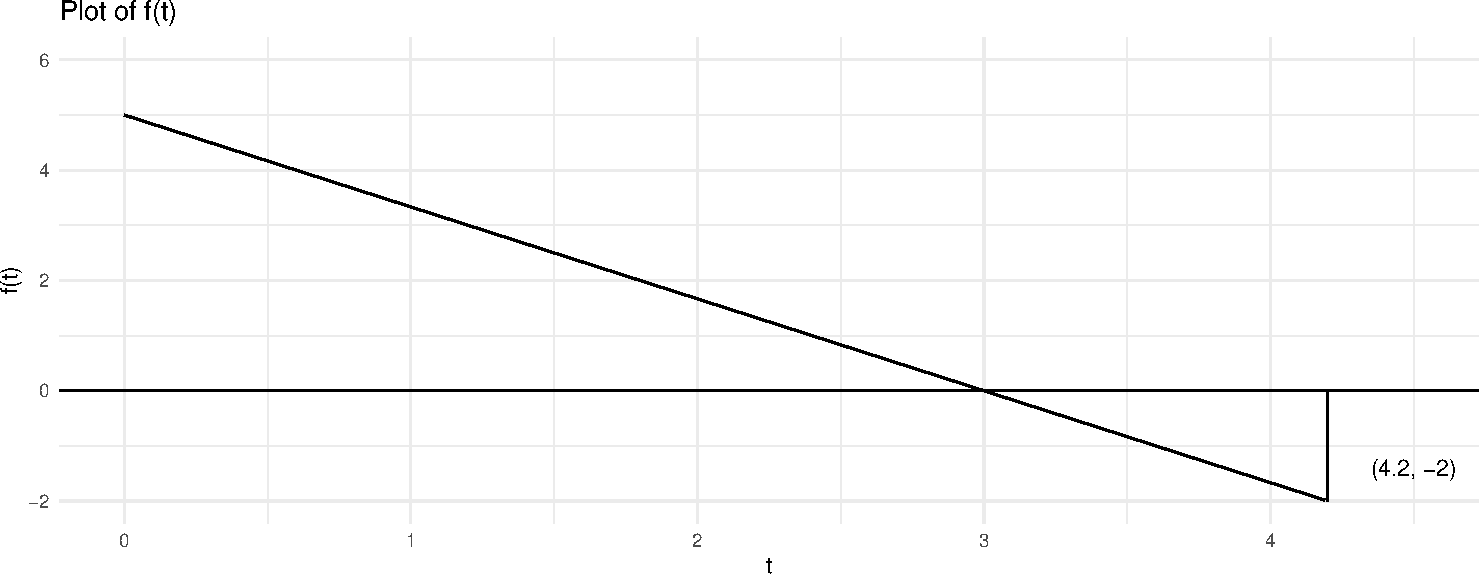
\includegraphics{laplace_transform_files/figure-latex/plot-function-1.pdf}

The plot above illustrates the behavior of the function \(f(t)\).

\hypertarget{representing-sub-signals-from-the-given-signal}{%
\subsection{Representing sub signals from the given
signal}\label{representing-sub-signals-from-the-given-signal}}

The above signal can be expressed as, \[f(t) = x(t)g(t)\]

\(x(t)\) can be represented graphically,

\begin{Shaded}
\begin{Highlighting}[]
\NormalTok{t\_values }\OtherTok{\textless{}{-}} \FunctionTok{seq}\NormalTok{(}\DecValTok{0}\NormalTok{, }\DecValTok{5}\NormalTok{, }\AttributeTok{by =} \FloatTok{0.01}\NormalTok{)}
\NormalTok{f\_values }\OtherTok{\textless{}{-}} \FunctionTok{f}\NormalTok{(t\_values)}

\NormalTok{df }\OtherTok{\textless{}{-}} \FunctionTok{data.frame}\NormalTok{(}\AttributeTok{t =}\NormalTok{ t\_values, }\AttributeTok{f =}\NormalTok{ f\_values)}
\FunctionTok{ggplot}\NormalTok{(df, }\FunctionTok{aes}\NormalTok{(}\AttributeTok{x =}\NormalTok{ t, }\AttributeTok{y =}\NormalTok{ f)) }\SpecialCharTok{+}
  \FunctionTok{geom\_line}\NormalTok{() }\SpecialCharTok{+}
  \FunctionTok{geom\_hline}\NormalTok{(}\AttributeTok{yintercept =} \DecValTok{0}\NormalTok{) }\SpecialCharTok{+}  
  \FunctionTok{annotate}\NormalTok{(}\StringTok{"text"}\NormalTok{, }\AttributeTok{x =} \FloatTok{4.2}\NormalTok{, }\AttributeTok{y =} \SpecialCharTok{{-}}\DecValTok{2}\NormalTok{, }\AttributeTok{label =} \StringTok{"(4.2, {-}2)"}\NormalTok{, }\AttributeTok{vjust =} \SpecialCharTok{{-}}\FloatTok{1.5}\NormalTok{, }\AttributeTok{hjust =} \SpecialCharTok{{-}}\FloatTok{0.5}\NormalTok{) }\SpecialCharTok{+}  
  \FunctionTok{xlim}\NormalTok{(}\DecValTok{0}\NormalTok{, }\FloatTok{4.5}\NormalTok{) }\SpecialCharTok{+} 
  \FunctionTok{ylim}\NormalTok{(}\SpecialCharTok{{-}}\DecValTok{2}\NormalTok{, }\DecValTok{6}\NormalTok{) }\SpecialCharTok{+} 
  \FunctionTok{labs}\NormalTok{(}\AttributeTok{title =} \StringTok{"Plot of ramp function x(t)"}\NormalTok{, }\AttributeTok{x =} \StringTok{"t"}\NormalTok{, }\AttributeTok{y =} \StringTok{"x(t)"}\NormalTok{) }\SpecialCharTok{+}
  \FunctionTok{theme\_minimal}\NormalTok{()}
\end{Highlighting}
\end{Shaded}

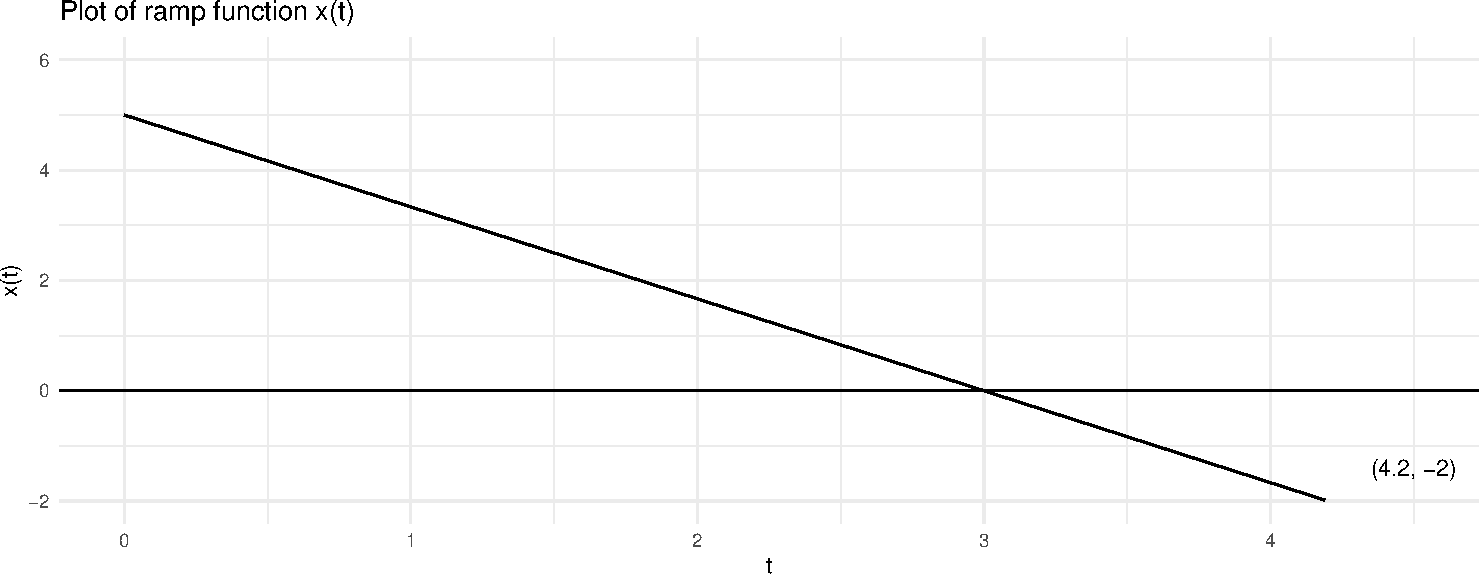
\includegraphics{laplace_transform_files/figure-latex/plot-function2-1.pdf}

Similarly, \(g(t)\) can be represented graphically,

\begin{Shaded}
\begin{Highlighting}[]
\NormalTok{step\_data }\OtherTok{\textless{}{-}} \FunctionTok{data.frame}\NormalTok{(}\AttributeTok{t =} \FunctionTok{c}\NormalTok{(}\DecValTok{0}\NormalTok{, }\FloatTok{4.2}\NormalTok{),}
                        \AttributeTok{g =} \FunctionTok{c}\NormalTok{(}\DecValTok{1}\NormalTok{, }\DecValTok{1}\NormalTok{))}

\CommentTok{\# Create the plot}
\FunctionTok{ggplot}\NormalTok{(step\_data, }\FunctionTok{aes}\NormalTok{(}\AttributeTok{x =}\NormalTok{ t, }\AttributeTok{y =}\NormalTok{ g)) }\SpecialCharTok{+}
  \FunctionTok{geom\_step}\NormalTok{(}\AttributeTok{direction =} \StringTok{"hv"}\NormalTok{) }\SpecialCharTok{+} 
  \FunctionTok{geom\_segment}\NormalTok{(}\FunctionTok{aes}\NormalTok{(}\AttributeTok{x =} \DecValTok{0}\NormalTok{, }\AttributeTok{y =} \DecValTok{0}\NormalTok{, }\AttributeTok{xend =} \DecValTok{0}\NormalTok{, }\AttributeTok{yend =} \DecValTok{1}\NormalTok{)) }\SpecialCharTok{+} 
  \FunctionTok{geom\_segment}\NormalTok{(}\FunctionTok{aes}\NormalTok{(}\AttributeTok{x =} \FloatTok{4.2}\NormalTok{, }\AttributeTok{y =} \DecValTok{0}\NormalTok{, }\AttributeTok{xend =} \FloatTok{4.2}\NormalTok{, }\AttributeTok{yend =} \DecValTok{1}\NormalTok{)) }\SpecialCharTok{+} 
  \FunctionTok{xlim}\NormalTok{(}\DecValTok{0}\NormalTok{, }\FloatTok{4.2}\NormalTok{) }\SpecialCharTok{+}  
  \FunctionTok{ylim}\NormalTok{(}\DecValTok{0}\NormalTok{, }\FloatTok{1.0}\NormalTok{) }\SpecialCharTok{+}  
  \FunctionTok{labs}\NormalTok{(}\AttributeTok{title =} \StringTok{"Unit Step Function g(t)"}\NormalTok{, }\AttributeTok{x =} \StringTok{"t"}\NormalTok{, }\AttributeTok{y =} \StringTok{"g(t)"}\NormalTok{) }\SpecialCharTok{+} 
  \FunctionTok{theme\_minimal}\NormalTok{()}
\end{Highlighting}
\end{Shaded}

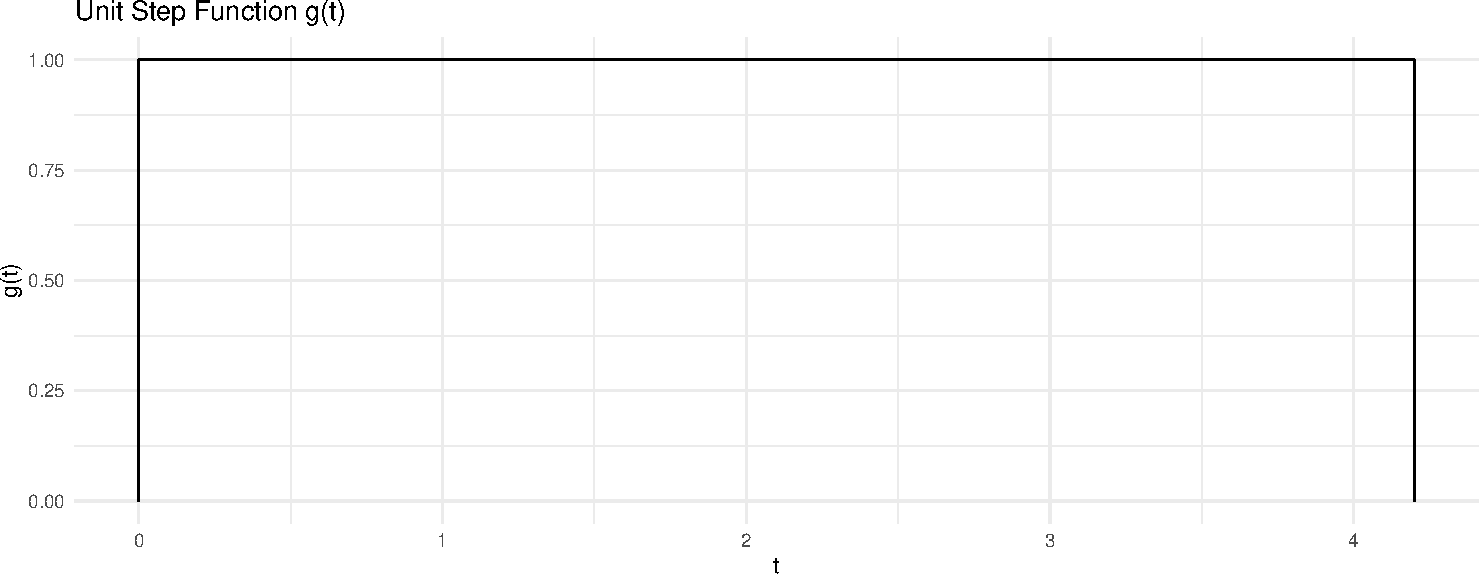
\includegraphics{laplace_transform_files/figure-latex/plot-function3-1.pdf}

\hypertarget{calculate-the-laplace-transform}{%
\subsection{Calculate the Laplace
Transform}\label{calculate-the-laplace-transform}}

The Laplace transform of \(f(t)\) is given by the formula:

\[ F(s) = \int_0^{\infty} e^{-st} f(t) dt \]

Substituting appropriate values for \(x(t)\) and \(g(t)\) in. \(f(t)\),
we get,

\(f(t) = [\frac{-5}{3}t + 5] [u(t) - u(t - 4.2)]\)

\(=\frac{-5}{3}t u(t) + \frac{5}{3}t u(t - 4.2) + 5u(t) - 5u(t - 4.2)\)

\(=\frac{-5}{3}t u(t) + \frac{5}{3}(t - 4.2 + 4.2)u(t - 4.2) + 5u(t) - 5u(t - 4.2)\)

\(=\frac{-5}{3}t u(t) + \frac{5}{3}(t - 4.2)u(t - 4.2) + 7u(t - 4.2) + 5u(t) - 5u(t-4.2)\)

\(=\frac{-5}{3}t u(t) + \frac{5}{3}(t - 4.2)u(t - 4.2) + 2u(t - 4.2) + 5u(t)\)\\

Hence,

\(F(s) = L[f(t)]\)
\[= \frac{-5}{3s^2} + \frac{5}{3s^2}e^{-4.2s} + \frac{5}{s}\] Which
simplfies to, \[=\frac{-5 + 5e^{-4.2s} + 6se^{-4.2s} + 15s}{3s^2}\]
Therefore,

\[L[f(t)] = \frac{-5 + 5e^{-4.2s} + 6se^{-4.2s} + 15s}{3s^2}\]

\hypertarget{conclusion}{%
\subsection{Conclusion}\label{conclusion}}

In this report, we've discussed the process of finding the Laplace
transform of the function \(f(t) = \left(-\frac{5}{3}\right)t + 5\).
We've plotted the function and outlined the manual calculation process
for finding its Laplace transform. Further numerical or symbolic
computations can be performed to obtain \(F(s)\) for specific values of
\(s\) if needed.

\hypertarget{acknowledgement}{%
\subsection{Acknowledgement}\label{acknowledgement}}

I would like to express my sincere gratitude to Professor Dr.~Niranjan K
R sir for granting me permission to carry out this report on Laplace
transform for network analysis. His guidance and support have been
invaluable throughout the process, and I am deeply thankful for the
opportunity to work on this AAT under his supervision.

\end{document}
